\documentclass{uonmathreport}

% loads already mathtools, graphicx,
% but you may want to add other packages, like
\usepackage{listings} % to include code in python see https://en.wikibooks.org/wiki/LaTeX/Source_Code_Listings
% other useful pagackes include booktabs, hyperref, amsthm, xcolor, todonotes, showkeys, ...
% see https://www.overleaf.com/learn 

% change the following to
% to \PJA = MATH4041, \PJS = MATH4042 or \DIS = MATH4001 (for BSc and MMAth)
% or \MSc (for all Msc dissertations)
\PJA

% adjust the following
\title{Title of the report goes here\\ and it may have several lines}
\author{Alvin Jonel De la Cruz Guerrero}
\academicyear{2022/23}
\supervisor{Dr. Your Supervisor}

% the following are irrelevant for Msc:
\assessmenttype{Review} % or Investigation

% the following are irrelevant for PJS, PJA, DIS:
% Msc: change it to G14PMD and Pure Mathematics, etc ...
\msccode{MATH4021}
\msctitle{Statistics}

% put your own definitions and shorthands here
\newcommand{\ZZ}{\mathbb{Z}}

\begin{document}

\maketitle

\begin{abstract}
The abstract of the report goes here. The abstract should state the
topic(s) under investigation and the main results or
conclusions. Methods or approaches should be stated if this is
appropriate for the topic. The abstract should be self-contained,
concise and clear. The typical length is one paragraph.
\end{abstract}

% Table of contents
\setcounter{tocdepth}{2}  % this will list subsections, but not subsubsections
\tableofcontents 
\newpage

\section{Introduction} \label{sec:intro}

The introductory section goes here. And remember the introduction
is the last thing you write.

% this is a comment in the file that won't appear in the output

The end of the introductory section would typically outline the
structure of the report. In this template, section \ref{sec:background}
gives the background of the topic, sections \ref{sec:my1} and
\ref{sec:my2} contain the bulk of the work and section
\ref{sec:conclusions} summarises and discusses what has been
achieved. Appendix \ref{app:rawdata} displays the raw data, and
certain technical calculations for section \ref{sec:my1} are deferred
to appendix \ref{app:calculations}.


\section{Background} \label{sec:_background}

\subsection{Finance}

A common problem in finance is to price financial derivatives, often referred just
as derivatives. In essence, derivatives are contracts set between parties 
whose value in time derives from the price of their underlying assets. A notorious
family of derivatives in financial markets are "options". Options
are contracts set between two parties in which the holder has the right 
to sell or buy, commonly referred as exercise, an underlying stock at a preestablished price, 
also known as "strike price", in the future. Options are referred as "call options" 
or as "put options" if the exercise position is to buy or to sell, respectively. 
Similarly, options are classified depending on their exercise style. In that regard,
the simplest of options are European options. European options give the right 
to exercise at the expiration date of the contract. Another well known type options 
are American options. American options give the right to exercise at any 
point in time between the beginning and expiration date of the contract. 
Let us define the payoff as

\begin{align}
  H(S,t) = \begin{cases}
    \max(S - K, 0) & \text{(call)}\\ 
     \max(K - S, 0) & \text{(put)}
   \end{cases}
\end{align}

where $K$ is the strike price, $S\in[0,\infty]$ is the stock price, and 
$t \in [0, T]$ is the current time. Note that $t$ is measure in years, $t=0$ and $t=T$
denotes the beginning of the contract and the expiration date, and
the region $[0,T]$ is the life span of the option. While an American option's payoff
is defined for all $(S,t)$, European options' payoff is only defined at $t=T$.   

Obviously, options give greater flexibility 
to holders by removing their exposure of a negative payoff which is why writers of 
the option charge a premium to the buyers at the time they enter the contract. 
The premium is often referred as the price or value of the option and the problem of finding this value is called option pricing. 
When pricing options, it is important to find the just price because 
otherwise the writer or buyer of the option could set some scheme in which option
will always be profitable to them. In other words, options pricing must follow
the principle of no-arbitrage. Therefore, we assume that the writer of the option
uses the premium to construct a portfolio consisting of $\phi_0$ units of the 
stock and invests $\psi_0$ units of cash into a risk-free asset such as US
tresury bill, certificate of deposit, or bank account. Then, the writer rebalanced
the portfolio $(\phi_0, \psi_0)$ to hedge any 
possible claims from the buyer of the option at any future time $0 < t \le T$. 
Therefore, at any time $t$, the writer holds a portfolio $(\phi(t), \psi(t))$ 
with value

\begin{equation}
  \Pi(t) = \phi(t)S(t) + \psi(t)B(t)
\end{equation}

Moreover, the portfolio is self-financing. In other words, the changes in the value
of the portfolio $V(t)$ depend on the changes in $S(t)$ and $B(t)$, and the current
portfolio $(\phi(t), \psi(t))$

\begin{equation}
  d\Pi(t) = \phi(t)dS(t) + \psi(t)dB(t)
\end{equation}

Finally, the value of an option must satisfy the following

\begin{equation}
  \Pi(t) = V(t)
\end{equation}

at any time $0 \le t \le T$.

The black schole model is built upon the self-financing portfolio hedging strategy 
and expresses a mathematical model for dynamics of option's price. 
The black schole model makes with some assumptions about the market. For complete
list of these assumptions look at (reference). We enumerates the one we believe 
are important for our task. First, the stock price $S(t)$ is a log-normal random
variable 

\begin{equation}
  dS = r(t)Sdt + \sigma(t) S dW
\end{equation}

where the risk-free interest $r(t)$ and the price volatility $\sigma(t)$ are 
deterministic functions of time during the life of the option. Secondly, the 
bank account $B(t)$ is a deterministic function of time

\begin{equation}
  dB = r(t)B(t)dt
\end{equation}

Finally, the stock does not pay dividends. From now on, we will assume that 
the risk-free interest rate and stock price volatility are constant during the 
life of the option. Later on, we will address the assumption about dividends.

By applying the black schole model to price European options, the famous black-schole 
PDE is obtained

\begin{equation}
  \begin{cases}
    \frac{\partial{V}}{\partial{t}} + \frac{1}{2}\sigma^{2} S^2 \frac{\partial^2{V}}{\partial{S^2}} + r S \frac{\partial{V}}{\partial{S}} - rV = 0 & \text{for $t\in[0,T)$ and $S\in[0, \infty)$} \\
    V(S, T) = H(S, T) & \text{for $S\in[0, \infty)$}
  \end{cases}
  \label{eq:background:finance:european_option_pde}
\end{equation}

where $V(S, t)$ is a deterministic function. For the derivation of 
(\ref{eq:background:finance:european_option_pde}), we reference to REFERENCE.

We previously mention that the one of the assumptions of the Black-Schole model is
that the underlying stock does not pay dividends. In most cases, assets such as stock
pay out dividends just a few times at year. Therefore, dividends are to be 
modelled discretely. However, there are certain assets that pay out a proportion
of the current asset price during and interval of time. Thus, in such cases, it is
useful to model dividends as a continuous yield. By arbitrage arguments [REFERENCES], it can be shown that the asset price with volatility $\sigma(t)$, rate of return $r(t)$,
and continuous dividend yield $\delta(S,t)$ paid at instant of time $dt$ is modeled as

\begin{align}
  dS = (r(t) - \delta(S, t))Sdt + \sigma(t) S dW
  \label{eq:background:finance:bs_price_model_with_dividends}
\end{align}

Similarly to
as we did for the risk-free interest rate and the volatility of the asset price,
we will assume that continuous dividends yield is as constant from now on. [REFERENCES]
show that applying the Black-Schole model under the price model (\ref*{eq:background:finance:bs_price_model_with_dividends}) to price European options,
we obtain the slightly modified version of (\ref*{eq:background:finance:european_option_pde})

\begin{equation}
  \begin{cases}
    \frac{\partial{V}}{\partial{t}} + \frac{1}{2}\sigma^{2} S^2 \frac{\partial^2{V}}{\partial{S^2}} + (r - \delta) S \frac{\partial{V}}{\partial{S}} - rV = 0 & \text{for $t\in[0,T)$ and $S\in[0, \infty)$} \\
    V(S, T) = H(S, T) & \text{for $S\in[0, \infty)$}
  \end{cases}
  \label{eq:chapter2:european_option_pde_with_dividens}
\end{equation}
 
Similarly, the Black-Schole model is applied to price American options. 
One important result is that the value of an American option $V_\text{Ame}(t)$ is
bounded from below by the payoff function

\begin{align}
  V_{\text{Am}}(S, t) \ge H(S, t) \qquad \text{for $t\in[0,T]$}
  \label{eq:background:american_options_price_lower_bound}
\end{align}

Moreover, the domain of $V(S,t)$ can be separated in the exercise region 

\begin{equation}
  \mathcal{S} := \{(S, t): V(S, t) = H(S, t) \}
\end{equation}

and the continuation region 

\begin{equation}
  \mathcal{C} := \{(S, t): V(S, t) > H(S, t) \}
\end{equation}

where the boundary of $\mathcal{C}$ is defined as

\begin{equation}
  \partial \mathcal{C} := \{(S, t): S = \bar{S}(t)\} 
\end{equation}

Lastly, the price dynamics of American options behaves as European options within
the continuation region. Since we know $V(S, t)$ at the stopping region, we only
need to solve $V(S,t)$ at continuation region and determine its boundary $\partial$
at the same time. Therefore, this is known as the free boundary problem formulation
of the American option pricing problem and is equivalent to solve.

\begin{align}
  \begin{cases}
  \frac{\partial{V}}{\partial{t}} + \frac{1}{2}\sigma^{2} S^2 \frac{\partial^2{V}}{\partial{S^2}} + (r - \delta)S \frac{\partial{V}}{\partial{S}} - rV = 0 & \text{for $(S, t) \in \mathcal{C}$} \\
  V(S, t) = H(S, t) & \text{for $(S,t)\in \partial\mathcal{C}$}
  \end{cases}
  \label{eq:background:finance:american_options_pde_free_boundary_problem}
\end{align}

Now, note that the bound of $V(S, t)$ in each region is
\begin{align*}
  &V(S, t) - H(S, t) > 0 \qquad \text{for all $(S,t) \in \mathcal{C}$} \\ 
  &V(S, t) - H(S, t) = 0 \qquad \text{for all $(S,t) \in \mathcal{S}$}
\end{align*}

Similarly, the bound of $\mathcal{L}_{\text{BS}}(V)$ is
\begin{align*}
  &\frac{\partial{V}}{\partial{t}} + \frac{1}{2}\sigma^{2} S^2 \frac{\partial^2{V}}{\partial{S^2}} + (r - \delta)S \frac{\partial{V}}{\partial{S}} - rV = 0 \qquad \text{for $(S,t) \in \mathcal{C}$} \\
  &\frac{\partial{V}}{\partial{t}} + \frac{1}{2}\sigma^{2} S^2 \frac{\partial^2{V}}{\partial{S^2}} + (r - \delta)S \frac{\partial{V}}{\partial{S}} - rV < 0 \qquad \text{for $(S,t) \in \mathcal{S}$}
\end{align*}

Therefore, grouping the bounds above we form a linear complementary system of equations

{
  \color{red}  
  \begin{align*}
    \begin{cases}
      \mathcal{L}_{\text{BS}}(V) \cdot [V(S,t) - H(S,t)] = 0 & \text{for all $(S,t)$} \\
      V(S, t) - H(S, t) \ge 0 & \text{for all $(S, t)$}\\
      \mathcal{L}_{\text{BS}}(V) \le 0 &  \text{for all $(S, t)$}\\
      V(S, T) = H(S, T) \\  
    \end{cases}
  \end{align*}
}

By combining the expression above with the lower bound (\ref*{eq:background:american_options_price_lower_bound}),
we obtain a linearly complementary system of equations

The system of equation (\ref*{eq:background:finance:american_options_pde_free_boundary_problem}) could
be reformulated as free a boundary problem, or as a linear complementary problem. To 
reframe the problem as free boundary problem, note that we know the value of $V(S,t)$
in the stopping region. Hence, we only need to solve the Black-Schole PDE at the
continuation region but with unknown boundary condition given by $S=\bar{S}(t)$. 
Finally, at the terminal condition the unknown boundary condition is given by 
$\bar{S}(T) = K$.

\begin{align}
  \begin{cases}
  \frac{\partial{V}}{\partial{t}} + \frac{1}{2}\sigma^{2} S^2 \frac{\partial^2{V}}{\partial{S^2}} + (r - \delta)S \frac{\partial{V}}{\partial{S}} - rV = 0 & \text{for $(S, t) \in \mathcal{C}$} \\
  V(S, t) = H(S, t) & \text{for all $(t, \bar{S}(t))$} \\
  S = \bar{S}(T)
  \end{cases}
  \label{eq:background:finance:free_boundary_problem}
\end{align}

The system (\ref{eq:background:finance:free_boundary_problem}) 
is the free boundary formulation for the pricing problem for American options.
A detailed derivation of (\ref{eq:background:finance:american_options_pde}) 
can be found at [REFERENCES].


The equation (\ref*{eq:background:finance:american_options_pde}) 
is a paraboblic PDE. Moreover, by applying the transformation,

\begin{align}
  S = Ke^x, \quad t = T - \frac{2\tau}{\sigma^2}, \quad q := \frac{2r}{\sigma^2}, \quad q_{\delta} := \frac{2(r-\delta)}{\sigma^2} & \\
  v(x, \tau) := V(S, t) = V\big(Ke^x, T - \frac{2\tau}{\sigma^2}\big) \\
  \alpha := \frac{1}{2}(q_{\delta} - 1) \quad \beta := \frac{1}{4}(q_{\delta} - 1)^2 + q  \\
  v(x, \tau) := e^{-(\alpha x + \beta \tau)}y(x, \tau)
\end{align}

the equation (\ref*{eq:background:finance:american_options_pde}) converts 
to the heat diffusion PDE.

\begin{equation}
  h(x, \tau) := \frac{H(S, t)}{K} = \begin{cases}
    \max(e^{x} - 1, 0)\\
    \max(1 - e^{x}, 0)
  \end{cases} 
\end{equation}

\begin{equation}
  \bar{x}(\tau) := \log{\bar{S}(t)} - \log{K} 
\end{equation}

\begin{align}
  \begin{cases}
    \frac{\partial y}{\partial \tau} = \frac{\partial^2 y}{\partial x^2} & \text{for $\tau\in[0,\frac{\sigma^2}{2}T)$ and $x\in(\bar{x}(t), \infty)$} \\
    y(x, \tau) = e^{(\alpha x + \beta \tau)}h(x, \tau) & \text{for $\tau\in[0, \frac{\sigma^2}{2}T]$ and $x\in(-\infty, \bar{x}(\tau)]$} \\
    \bar{x}(0) = 0
  \end{cases}
  \label{eq:background:finance:american_option_heat_equation}
\end{align}

We can reformulate equation (\ref*{eq:background:finance:american_option_heat_equation})
as:

\begin{equation}
  g := e^{\alpha x + \beta \tau}h(x, \tau)
\end{equation}

\begin{align}
  \begin{cases}
    \big(\frac{\partial y}{\partial \tau} - \frac{\partial^2 y}{\partial x^2}\big)(y  - g) =0 \\
    \frac{\partial y}{\partial \tau} - \frac{\partial^2 y}{\partial x^2} \ge 0 \quad y - g \ge 0 \\
    y(x, 0) = g(x, 0)
  \end{cases}
\end{align}


By exploring the geometric properties of the value function $V(S,t)$, 
we can determine useful conditions that will later help on in solving the equation 
(\ref*{eq:background:finance:american_options_pde}). Firstly, at
any given time $0 \le t \le T$, American options match the linear segment of the payoff
function within the stopping region. Therefore, we could say that 

\begin{align}
  \frac{\partial V}{\partial S}(S, t) =  \begin{cases}
    -1 & \text{(put)} \\ 
    1 & \text{(call)}
  \end{cases}
  \label{eq:background:finance:american_option_left_boundary}
\end{align}

Moreover, as the price goes to infinity the value of the option tends to zero

\begin{align}
  \lim_{S \rightarrow \infty}V(S, t) = 0 
  \label{eq:background:finance:american_option_stopping_right_boundary}
\end{align}


\subsection{Numerical methods for the heat diffusion PDE}

Pricing American options requires using numerical methods. The Black-Schole PDE 
in (XXX) can be converted to the heat diffusion equation


Therefore, we focus on analyzing the numerical solution of the heat diffusion equation. 
Suppose the equation (XXX) is defined within the rectangular region $[x_{\text{min}}, x_{\text{max}}]\times[\tau_{\text{min}}, \tau_{\text{max}}]$.
By discretizing uniformly along the spatial direction $x$ and temporal direction $\tau$,

\begin{align}
  M &:= \frac{x_{\text{max}} - x_{\text{min}}}{\Delta x} \\ 
  N &:= \frac{\tau_{\text{max}} - \tau_{\text{min}}}{\Delta \tau} \\ 
  x_i &:= x_{\text{min}} + i\Delta x & \text{for $i = 0,\dots, M$} \\
  \tau_i &:= \tau_{\text{min}} + i{\Delta \tau} & \qquad \text{for $i = 0,\dots, N$}
\end{align}

where $\Delta x$ and $\Delta \tau$ are the distance between two consecutive points,
then, the grid is defined as the discrete region. 

\begin{align}
  \mathcal{G} := \{(x_i, \tau_j): (i, j) \in \{0,\dots,M\}\times\{0,\dots,N\}\}
\end{align}

Thus, solving numerically the equation (XXX) means finding an approximation for $y(x_i, \tau_n)$ at every 
$(x_i, \tau_n)$ within the grid $\mathcal{G}$,

\begin{align}
  y^{n}_i \approx y(x_i,\tau_n)
\end{align}

To obtain such approximation, we rely on central difference approximations (REFERENCE).

\begin{align}
  f'(x_i) &= \frac{f_{i+1} - f_{i}}{h} + O(h) \\
  f'(x_i) &= \frac{f_{i+1} - f_{i-1}}{2h} + O(h^2) \\
  f''(x_i) &= \frac{f_{i+1} - 2f_{i} + f_{i-1}}{h^2} + O(h^2)
\end{align}

\subsubsection{Explicit scheme}

An explicit scheme is one where we approximate the time partial derivative using
a forward difference approximation. Hence, the PDE in (XXX) is approximated as

\begin{equation}
  \frac{y^{n+1}_{i} - y^{n}_{i}}{\Delta \tau} = \frac{y^{n}_{i-1} - 2y^{n}_{i} + y^{n}_{i+1}}{(\Delta x)^2}
\end{equation}

By rearranging the terms,

\begin{equation}
  \lambda := \frac{\Delta \tau}{(\Delta x)^2}
\end{equation}

\begin{equation}
  y^{n+1}_i = \lambda y^{n}_{i-1} + (1 - 2\lambda)y^{n}_{i} + \lambda y^{n}_{i+1}
\end{equation}

It is shown by reference [REFERENCE] that method (XXX) is stable and consistent 
under the following condition

\begin{equation}
  0 < \Delta \tau \le \frac{(\Delta x)^2}{2}
\end{equation}

Moreover, the method has order of convergence $O(\Delta \tau, (\Delta x)^{2})$.

\subsubsection{Implicit scheme}

The implicit scheme approximates the time derivative using a backward difference

\begin{equation}
  \frac{y^{n+1}_{i} - y^{n}_{i}}{\Delta \tau} = \frac{y^{n+1}_{i-1} - 2y^{n+1}_{i} + y^{n+1}_{i+1}}{(\Delta x)^2}
\end{equation}

\begin{equation}
  y^{n+1}_{i} - \lambda (y^{n+1}_{i-1} - 2y^{n+1}_{i} + y^{n+1}_{i+1}) = y^{n}_{i}  
\end{equation}

\begin{equation}
  K := \begin{bmatrix}
    2 & -1     & & 0 \\ 
   -1 & \ddots & \ddots \\
      & \ddots & \ddots & \ddots \\
    0 & & \ddots & \ddots & \\
  \end{bmatrix} 
\end{equation}

\begin{equation}
  (I + \lambda K)\boldsymbol{y}^{n+1} = \boldsymbol{y}^{n}
\end{equation}

\subsubsection{Theta method}

\begin{equation}
  \frac{y^{n+1}_{i} - y^{n}_{i}}{\Delta \tau} = (1-\theta)\frac{y^{n}_{i-1} - 2y^{n}_{i} + y^{n}_{i+1}}{(\Delta x)^2} +  \theta\frac{y^{n+1}_{i-1} - 2y^{n+1}_{i} + y^{n+1}_{i+1}}{(\Delta x)^2}
\end{equation}

\begin{equation}
  y^{n+1}_{i} - \lambda\theta(y^{n+1}_{i-1} - 2y^{n+1}_{i} + y^{n+1}_{i+1}) =  y^{n}_{i} + (1-\theta)\lambda(y^{n}_{i-1} - 2y^{n}_{i} + y^{n}_{i+1})
\end{equation}

\begin{equation}
  (1 + \lambda\theta K)\boldsymbol{y}^{n+1} = (1-\lambda\theta K)\boldsymbol{y}^{n} 
\end{equation}

\section{Front fixing method}

\subsection{Inverse transformation}

\begin{equation}
    \frac{\partial{V}}{\partial{t}} + \frac{1}{2}\sigma^{2} S^2 \frac{\partial^2{V}}{\partial{S^2}} + (r - \delta) S \frac{\partial{V}}{\partial{S}} - rV = 0 \quad \text{for $S > \bar{S}(t)$ and $0 \le t < T$}
\end{equation}

\begin{equation}
    V(S, t) = K - S \quad  \text{for $0 \le S \le \bar{S}(t)$ and $0 \le t < T$}
\end{equation}

\begin{equation}
    V(S, T) = \max(K - S, 0) \quad \text{for $S \ge 0$}
\end{equation}

\begin{equation}
    \frac{\partial{V}}{\partial{S}}(\bar{S}(t), t) = -1
\end{equation}

\begin{equation}
    \lim_{S\rightarrow \infty} V(S, t) = 0
\end{equation}

\begin{equation}
    \bar{S}(T) = K
\end{equation}

In order for remove the free boundary in the system of equation, the following 
transformation is used:

\begin{equation}
    x = \frac{S}{\bar{S}(t)}
\end{equation}

Next,

\begin{equation}
    v(x, t) := V(x\bar{S}(t), t) = V(S, t)
\end{equation}


By computing the partial derivatives of V with respect to S and t

\begin{equation}
    \frac{\partial{V}}{\partial{t}} =  \frac{\partial{v}}{\partial{t}} + \frac{\partial{v}}{\partial{x}} \frac{\partial{x}}{\partial{t}} 
    = \frac{\partial{v}}{\partial{t}} - x\frac{\bar{S}^\prime(t)}{\bar{S}(t)}\frac{\partial{v}}{\partial{x}} 
\end{equation}

\begin{equation}
    \frac{\partial{V}}{\partial{S}} = \frac{\partial{v}}{\partial{x}} 
    \frac{\partial{x}}{\partial{S}} = 
    \frac{1}{\bar{S}(t)} \frac{\partial{v}}{\partial{x}}
\end{equation}

\begin{equation}
    \frac{\partial^2{V}}{\partial{S^2}} =
    \frac{1}{\bar{S}(t)^2} \frac{\partial^2{v}}{\partial{x}^2}
\end{equation}

an expression for (3.1) with respect to $x$ is derived:

\begin{equation}
    \frac{\partial{v}}{\partial{t}} + \frac{1}{2}\sigma^{2} x^2 \frac{\partial^2{v}}{\partial{x}^2} + \bigg[(r - \delta) - \frac{\bar{S}^\prime(t)}{\bar{S}(t)}\bigg]x\frac{\partial{v}}{\partial{x}} - rv = 0 \quad \text{for $x > 1$ and $0 \le t < T$}
\end{equation}

Similarly, (3.2) is reformulated in term of x to:

\begin{equation}
    v(x, t) = K - x\bar{S}(t) \quad  \text{for $0 \le x \le 1$ and $0 \le t < T$}
\end{equation}

Next, the terminal condition (3.3) is re-written with respect of x:

\begin{equation}
    v(x, T) = \max(K - x\bar{S}(T), 0) = K \max(1 - x, 0) = 0 \quad \text{for $x \ge 1$}
\end{equation}

Finally, the left and right boundary conditions are given with respect to x:

\begin{equation}
    \frac{\partial{v}}{\partial{x}}(x, t) = -\bar{S}(t)
\end{equation}

\begin{equation}
    \lim_{x \rightarrow \infty} v(x, t) = 0
\end{equation}

In summary, a non linear system of PDEs is obtained:

\begin{equation}
    \frac{\partial{v}}{\partial{t}} + \frac{1}{2}\sigma^{2} x^2 \frac{\partial^2{v}}{\partial{x}^2} + \bigg[(r - \delta) - \frac{\bar{S}^\prime(t)}{\bar{S}(t)}\bigg]x\frac{\partial{v}}{\partial{x}} - rv = 0 \quad \text{for $x > 1$ and $0 \le t < T$}
\end{equation}

\begin{equation}
    v(x, t) = K - x\bar{S}(t) \quad  \text{for $0 \le x \le 1$ and $0 \le t < T$}
\end{equation}

\begin{equation}
    v(x, T) = 0 \quad \text{for $x \ge 1$}
\end{equation}

\begin{equation}
    \frac{\partial{v}}{\partial{x}}(x, t) = -\bar{S}(t)
\end{equation}

\begin{equation}
    \lim_{x \rightarrow \infty} v(x, t) = 0
\end{equation}

\begin{equation}
    \bar{S}(T) = K
\end{equation}

\section{A section} \label{sec:background}

References can be for example
textbooks \cite{bott-tu,haw-ell,wolf,alling-greenleaf,hatcher},
conventional journal articles \cite{wheeler-geon,dewitt-can},
conventional journal articles that are also available at an e-print
server \cite{krasnov-louko,barrett-dawe}, electronic journal
articles \cite{poisson-livrev}, articles in conference proceedings
\cite{poisson-gr17}, PhD theses \cite{giulini-thesis,langlois-thesis}
or websites \cite{ligo-site}. This template orders the references by
their first citation, cites them by their number and keeps any
footnotes\footnote{Such as this.} separate from the references. Other
citation practices exist: Your supervisor can advise as to what is
appropriate for your topic.

\section{Another section} \label{sec:my1}

\subsection{A subsection} \label{subsec:theory}

Subsections may be used. Use a clear structure in your report.

We denote the set of real numbers by
$\mathbb{R}$, the set of integers by $\ZZ$ and the set of complex
numbers by $\mathbb{C}$. Our analysis is based on the equation
$e^{\pi i} = -1$ and the relation
\begin{equation}
  \frac{2}{4} = \frac{1}{2}   \label{eq:myeq1}
\end{equation} % no empty line after this
which we verify in the appendix \ref{app:calculations}.
Useful consequences are
\begin{align}
  \frac{4}{8} &= \frac{1}{2} \\
  \frac{4}{12} + \frac{1}{\Gamma(s)}\int_0^{\infty} \frac{t^{s-1}}{e^t-1} dt
     &= \frac{1}{3} +\sum_{n=1}^{\infty} \frac{1}{n^s}\\
  \frac{2}{10} &= \frac{1}{5} 
\end{align}
For any $0\neq a\in \ZZ$, the equality
\begin{equation*} % * for no numbering
 \frac{2 a}{4 a} = \frac{1}{2}
\end{equation*}
follows from equation \eqref{eq:myeq1}.

\subsection{Another subsection} \label{subsec:application}

\subsubsection{A subsubsection} \label{subsubsec:red}

Sometimes subsubsections may be appropriate.

\subsubsection{Another subsubsection} \label{subsubsec:green}



This could contain a table of interesting numbers
\begin{center}
  \begin{tabular}{r|cccccc}
    $n$   & 1 & 2 & 3 & 4 & 5 & 6 \\ \hline
    $F_n$ & 1 & 1 & 2 & 3 & 5 & 8 \\
    $B_n$ & $\tfrac{1}{2}$ & $\tfrac{1}{6}$ & 0 & $-\tfrac{1}{30}$ & 0 &  $\tfrac{1}{42}$ \\
    $p_n$ & 2 & 3& 5& 7 & 11 & 13 \\
  \end{tabular}
\end{center}

\section{Yet another section} \label{sec:my2}

Graphics can be included. Figure \ref{fig:bsd} shows an example.
Learn about floats and pictures in the \LaTeX\ wikibook to place
the figures at the right place.
%
\begin{figure}
 \begin{center}
   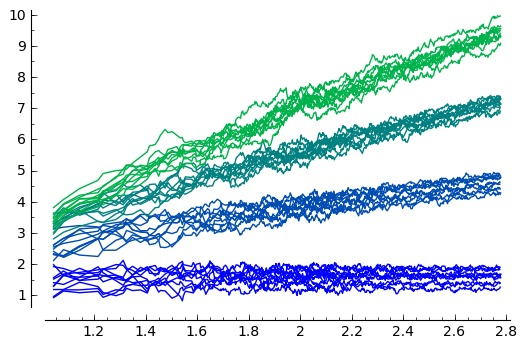
\includegraphics[width=0.7\textwidth]{bsd.jpg}
 \end{center}
 \caption{Oh look, something happens here !}
 \label{fig:bsd}
\end{figure}

\section{Conclusions} \label{sec:conclusions}

Further help on \LaTeX\ can be found easily on the internet. The \LaTeX\
wikibook\footnote{\tt http://en.wikibooks.org/wiki/LaTeX} contains a lot.
For instance you would find there how to type theorems and proofs nicely.
Or how to include source code written in some programming language like
python. There are long lists available with all sorts of common
mathematical symbols like $\xi$, $\nabla$, $\infty$, $\log$, $\iff$, etc.

\newpage

\appendix

\section{Raw data} \label{app:rawdata}

Material that needs to be included but would distract from the main
line of presentation can be put in appendices.
Examples of such material are raw
data, computing codes and details of calculations.

But note tha the maximal number of pages includes the appendix and the references.

\section{Calculations for section \ref{sec:my1}} \label{app:calculations}

In this appendix we could verify equation \eqref{eq:myeq1} or present the code that was used. 
\begin{lstlisting}[language=Python]
def gcd(a,b):
    """
    Return the greatest common divisor
    of a and b 
    """
    while b > 0:
        (a, b) = (b, a % b)
    return a
\end{lstlisting}
 
\newpage

\begin{thebibliography}{99} % alternatively use BibTeX

\bibitem{alling-greenleaf}
N.~L. Alling and N.~Greenleaf,
{\it Foundations of the Theory of Klein Surfaces\/},
Lecture Notes in Mathematics Vol.~219
(Springer, Berlin, 1971).

\bibitem{barrett-dawe}
J.~W. Barrett and R.~A. Dawe Martins,
``Non-commutative geometry and the standard model vacuum'',
{\it J. Math.\ Phys.\ \bf 47}, 052305 (2006).
(arXiv:hep-th/0601192)

\bibitem{bott-tu}
R.~Bott and L.~W. Tu,
{\it Differential Forms in Algebraic Topology\/}
(Springer, New York, 1982).

\bibitem{dewitt-can}
B.~S. DeWitt,
``Quantum theory of gravity. I. The canonical theory'',
{\it Phys.\ Rev.\ \bf 160}, 1113--1148
(1967).

\bibitem{giulini-thesis}
D.~Giulini,
``3-manifolds in canonical quantum gravity'',
PhD Thesis,
University of Cambridge (1990).

\bibitem{hatcher}
A.~Hatcher,
{\it Algebraic Topology\/}
(Cambridge University Press, Cambridge, 2002),
Proposition 1.40 and Exercise 1.3.24.

\bibitem{haw-ell}
S.~W. Hawking and G.~F.~R. Ellis,
{\it The Large Scale Structure of Space-Time\/}
(Cambridge University Press, Cambridge, 1973).

\bibitem{krasnov-louko}
K.~Krasnov and J.~Louko,
``$\mathrm{SO}_0(1,d+1)$ Racah coefficients: Type I representations'',
{\it J. Math.\ Phys.\ \bf 47}, 033513 (2006).
(arXiv:math-ph/0502017)

\bibitem{langlois-thesis}
P.~Langlois,
``Imprints of spacetime topology in the Hawking-Unruh effect'',
PhD Thesis, University of Nottingham (2005).
(arXiv: gr-qc/0510127)

\bibitem{poisson-livrev}
E.~Poisson,
``The motion of point particles in curved spacetime'',
{\it Living Rev.\ Relativity \bf 7} 6 (2004),
URL : \texttt{http://www.livingreviews.org/lrr-2004-6} (cited on 31 August 2006).
(arXiv: gr-qc/0306052)

\bibitem{poisson-gr17}
E.~Poisson,
``The gravitational self-force'',
in
{\it Proceedings of the
17th International Conference on General
Relativity and Gravitation\/} (Dublin, Ireland, July 18--23, 2004),
edited by
P.~Florides, B.~Nolan and A.~Ottewill
(World Scientific, Singapore, 2005) 119--141.
(arXiv:gr-qc/0410127)

\bibitem{wheeler-geon}
J.~A. Wheeler,
``Geons'',
{\it Phys.\ Rev.\ \bf 97}, 511--536
(1955).

\bibitem{wolf}
J.~A. Wolf,
{\it Spaces of Constant Curvature\/},
5th edition
(Publish or Perish, Wilmington, 1984).


\bibitem{ligo-site}
Website \texttt{http://www.ligo.caltech.edu/},
visited 14 August 2007.

\end{thebibliography}

\end{document}
